\chapter{Analisi architetturale di Delaire}
\nocite{Delaire1981,Cudia1991}

L'analisi cefalometrica proposta da Delaire è un'analisi architettonica e strutturale che considera linee verticali e orizontali tracciate a partire da punti di repere anatomici non convenzionali. Essa mira a chiarire il mutuo equilibrio tra le varie strutture ossee del cranio e della faccia.\\
Per poter utilizzare tale analisi sarà necessario avere una buona teleradiografia comprendente l'intera calotta cranica.

Si distinguono le strutture craniche da quelle mascellari, le prime individuate dalle sigle da C1 a C4, le seconde da CF1 a CF8, rispettivamente \emph{linee craniche} e \emph{linee cranio-facciali}.

\section{Analisi del cranio}

\begin{figure}[!ht]
\centering
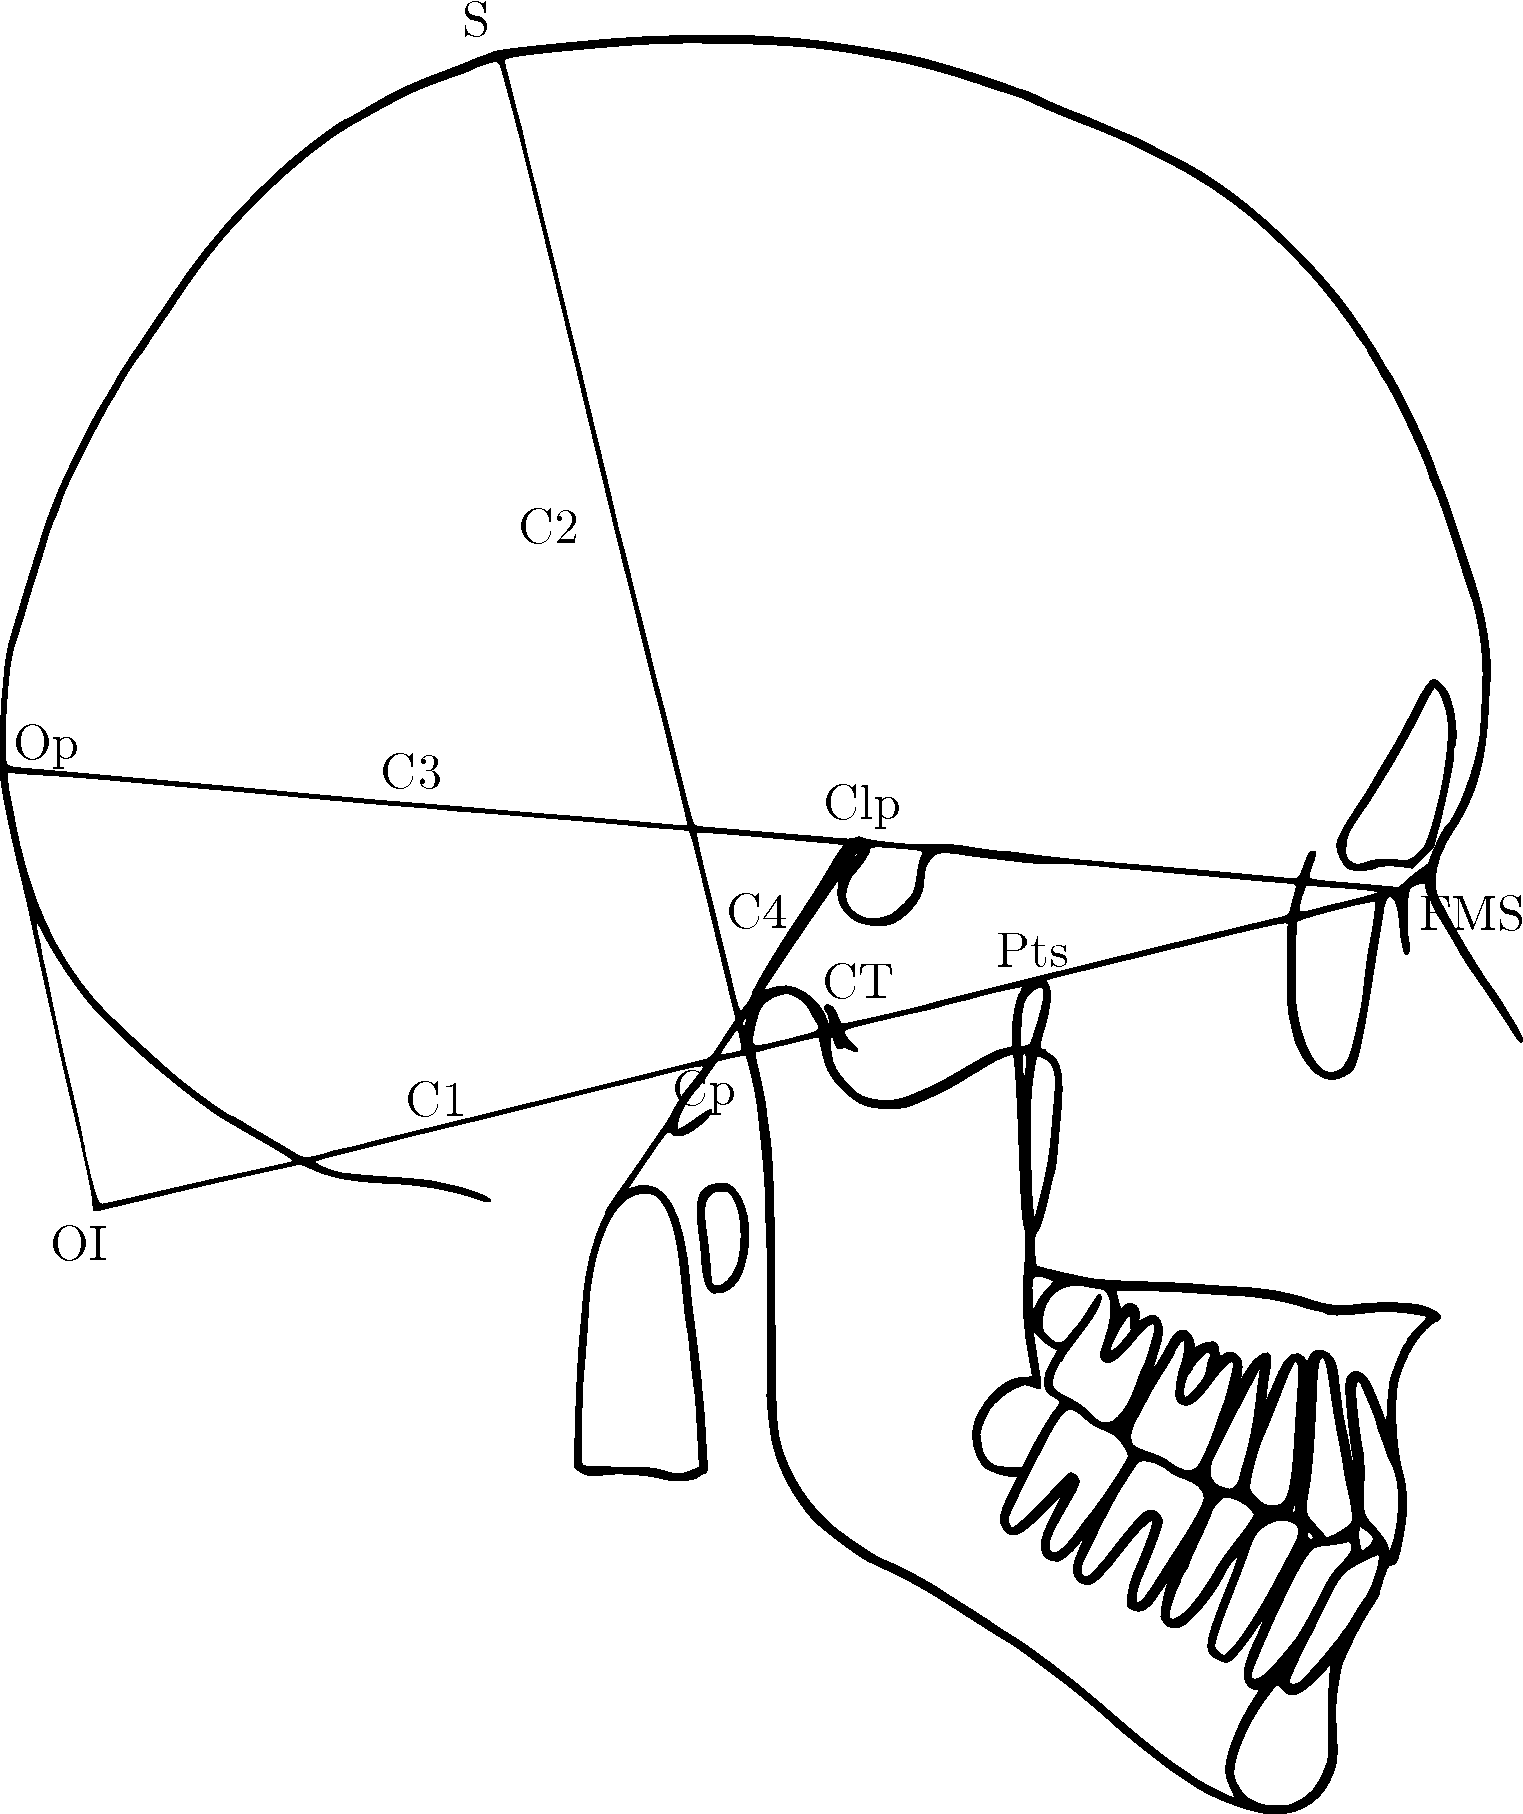
\includegraphics[width=.5\textwidth]{./images/delaire_craniali.pdf}
\caption{Linee craniche secondo Delaire}
\label{fig:delaire_craniche}
\end{figure}

\paragraph{Linea della base cranio-facciale} o \textbf{C1}, rappresenta il limite cranio-facciale, e viene tracciata dal punto \punto{FMS} (sutura fronto-mascellare), passante da \punto{CT} (punto temporo-condilare), ossia il punto inferiore della superficie postero-inferiore del tubercolo articolare del temporale. Tale linea viene poi estesa fino al punto \punto{OI} (occipitale inferiore), che è l'intersezione tra \textbf{C1} e la sua perpendicolare tangente alla superficie esterna dell'osso occipitale. \\ L'intersezione tra \textbf{C1} e la superficie posteriore del condilo definisce il punto \punto{Cp}. Normalmente, \punto{Cp} è posizionato a metà strada tra \punto{FMS} e \punto{OI}. Questo divide \textbf{C1} in due segmenti uguali, denominati rispettivamente \emph{area cranio-spinale} e \emph{area cranio-facciale}. Il tratto \piano{FMS}{Cp} interseca la parte superiore della fessura pterigomascellare in \punto{Pts}. In pazienti con un buon equilibrio cefalometrico, \piano{FMS}{Pts} e \piano{Pts}{Cp} stanno in un rapporto di 3:2.

\paragraph{Altezza cranica} o \textbf{C2}, è perpendicolare a \textbf{C1} nel suo punto centrale (normalmente \punto{Cp}), e interseca la calotta cranica in un punto \punto{SC}. Normalmente, \punto{SC} è il punto cranico più distante da \textbf{C1}, e \punto{SC} risulta essere la sommità del cranio. La lunghezza di \textbf{C2} è normalmente tra il 75 e l'85\% di \textbf{C1}. \\ Se \textbf{C2} non è tangente al margine posteriore del condilo si può fare subito una considerazione sul mancato equilibrio tra l'area cranio-spinale e l'area cranio-facciale: se passa al davanti sarà a favore della prima, per esempio nelle terze classi a crescita verticale; se passa al di dietro sarà a favore della seconda, ad esempio nei casi di terza classe a crescita orizzontale, nelle retrognazie e nei deep-bite.

\paragraph{Linea superiore della base cranica} o \textbf{C3}, viene tracciata dal punto \punto{FMS}, passante per l'apice del processo clinoideo \punto{Clp}, viene estesa posteriormente fino alla superficie esterna dell'osso occipitale, al punto \punto{OP} (punto occipitale posteriore). Di norma il segmento \piano{FMS}{Clp} è approssimativamente parallelo alla lamina cribrosa dell'etmoide, e passa vicino al processo clinoideo anteriore e il tubercolo ipofisario; il punto \punto{OP} risulta essere molto vicino alla perpendicolare a \textbf{C1} registrata in \punto{OI}.\\
L'angolo tra questa linea e \textbf{C1} è normalmente di 22°.

\paragraph{Linea del clivus} o \textbf{C4}, è formata dal punto \punto{Clp} alla parte postero-inferiore o all'apice del dente dell'epistrofeo. Normalmente, questa linea risulta essere tangente alla sella turcica, la superficie cerebrale dell'osso baso-occipitale e il basion, ed è molto vicina, e a volte tangente, alla superficie postero-superiore del condilo mandibolare.

\section{Analisi facciale}

\begin{figure}[!ht]
\centering
\subfloat[][]
   {\label{fig:delaire_bilancio_anteroposteriore}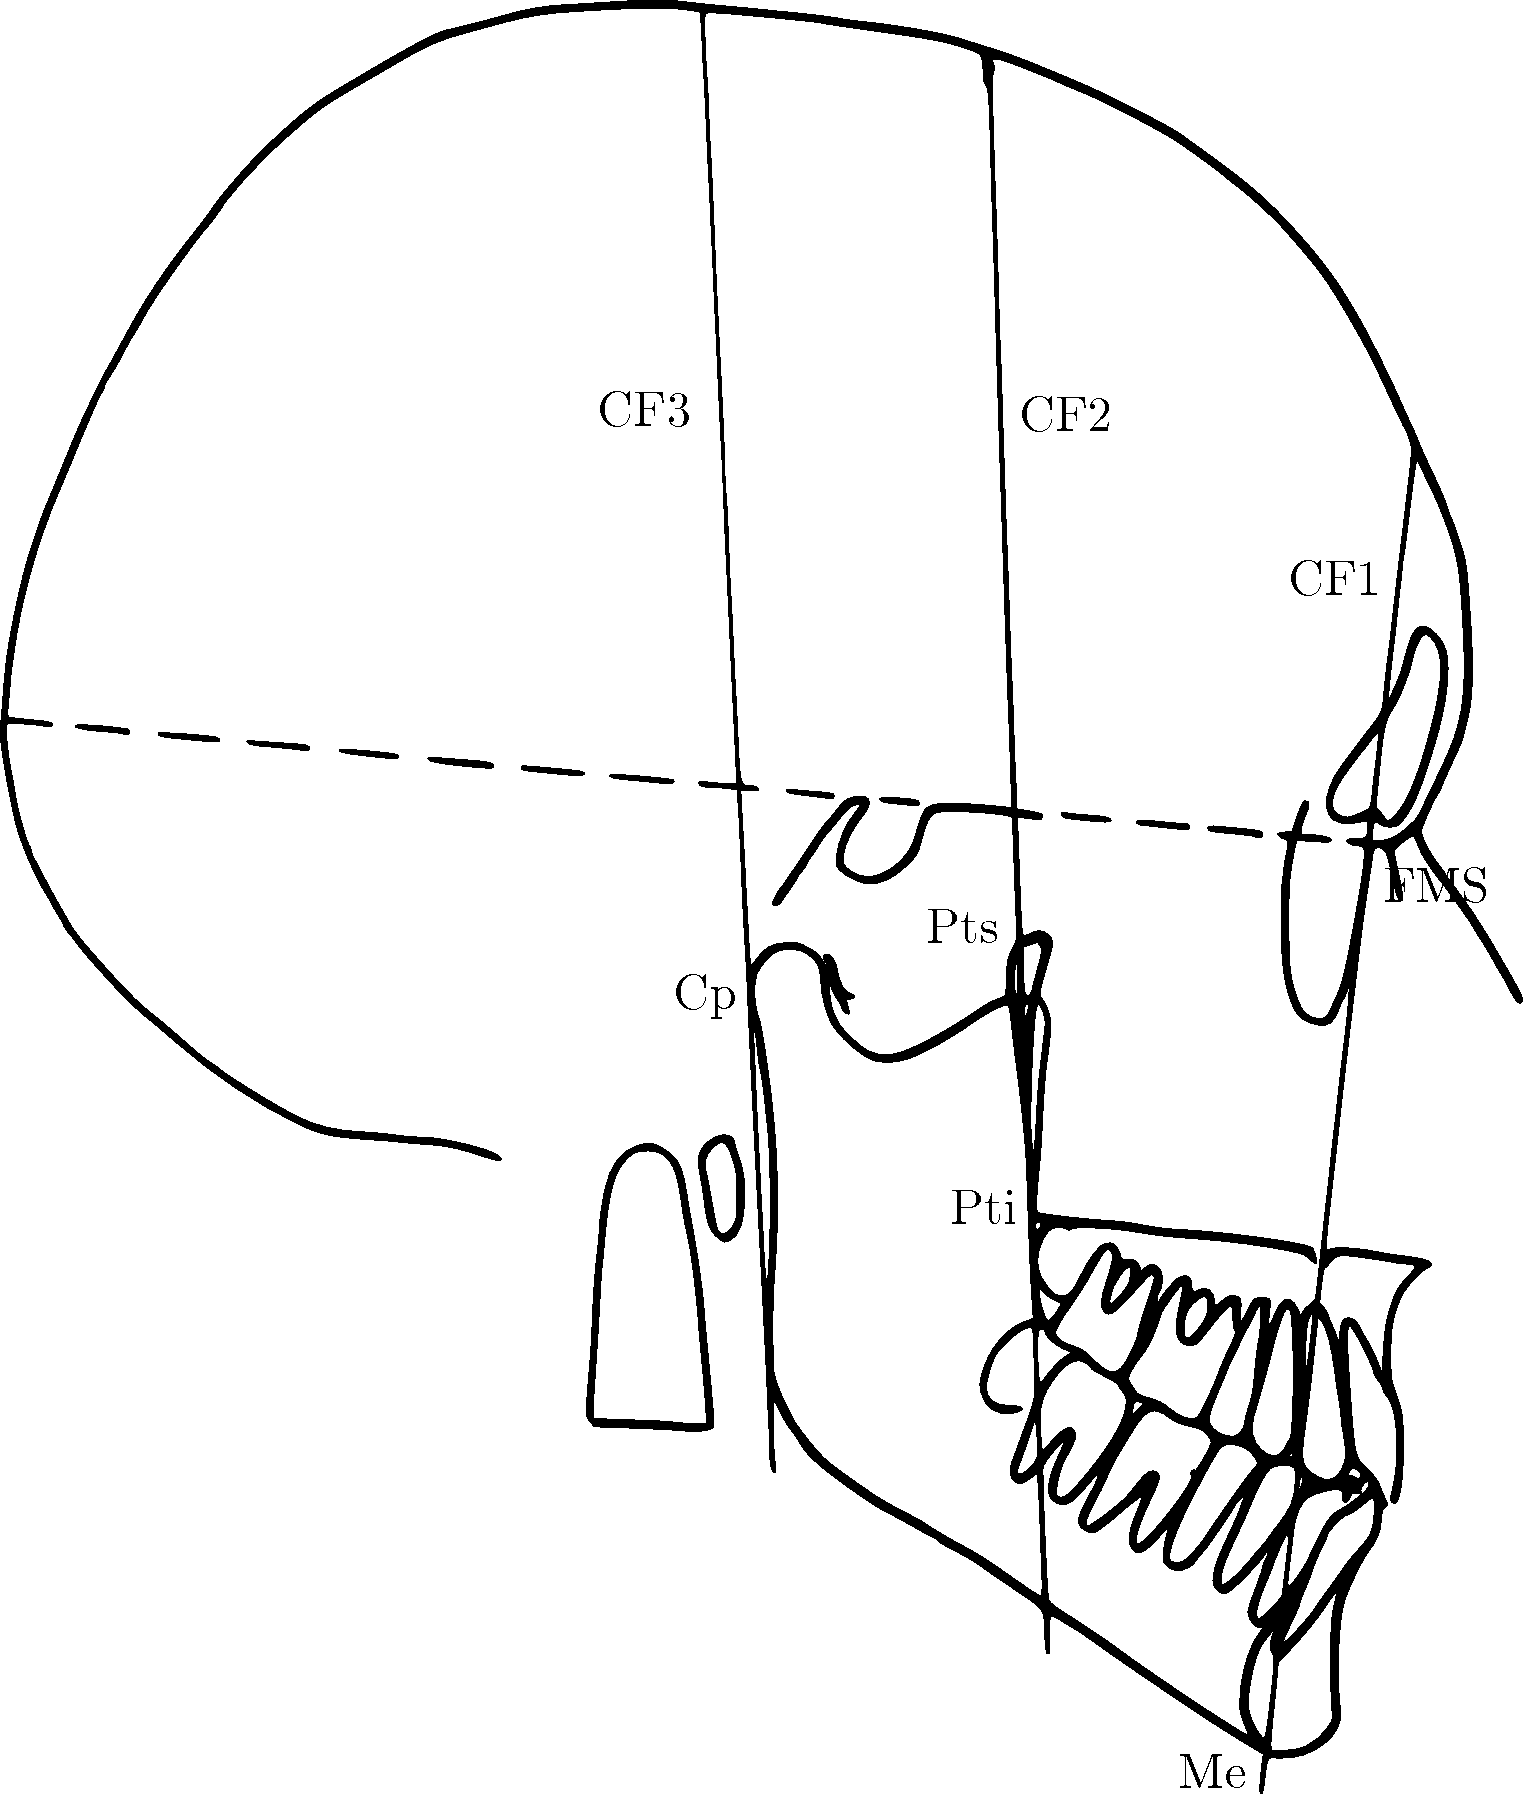
\includegraphics[width=.4\textwidth]{./images/delaire_bilancio_anteroposteriore.pdf}}
\hspace{3em}
\subfloat[][]
   {\label{fig:delaire_bilancio_palatoocclusomandibolare}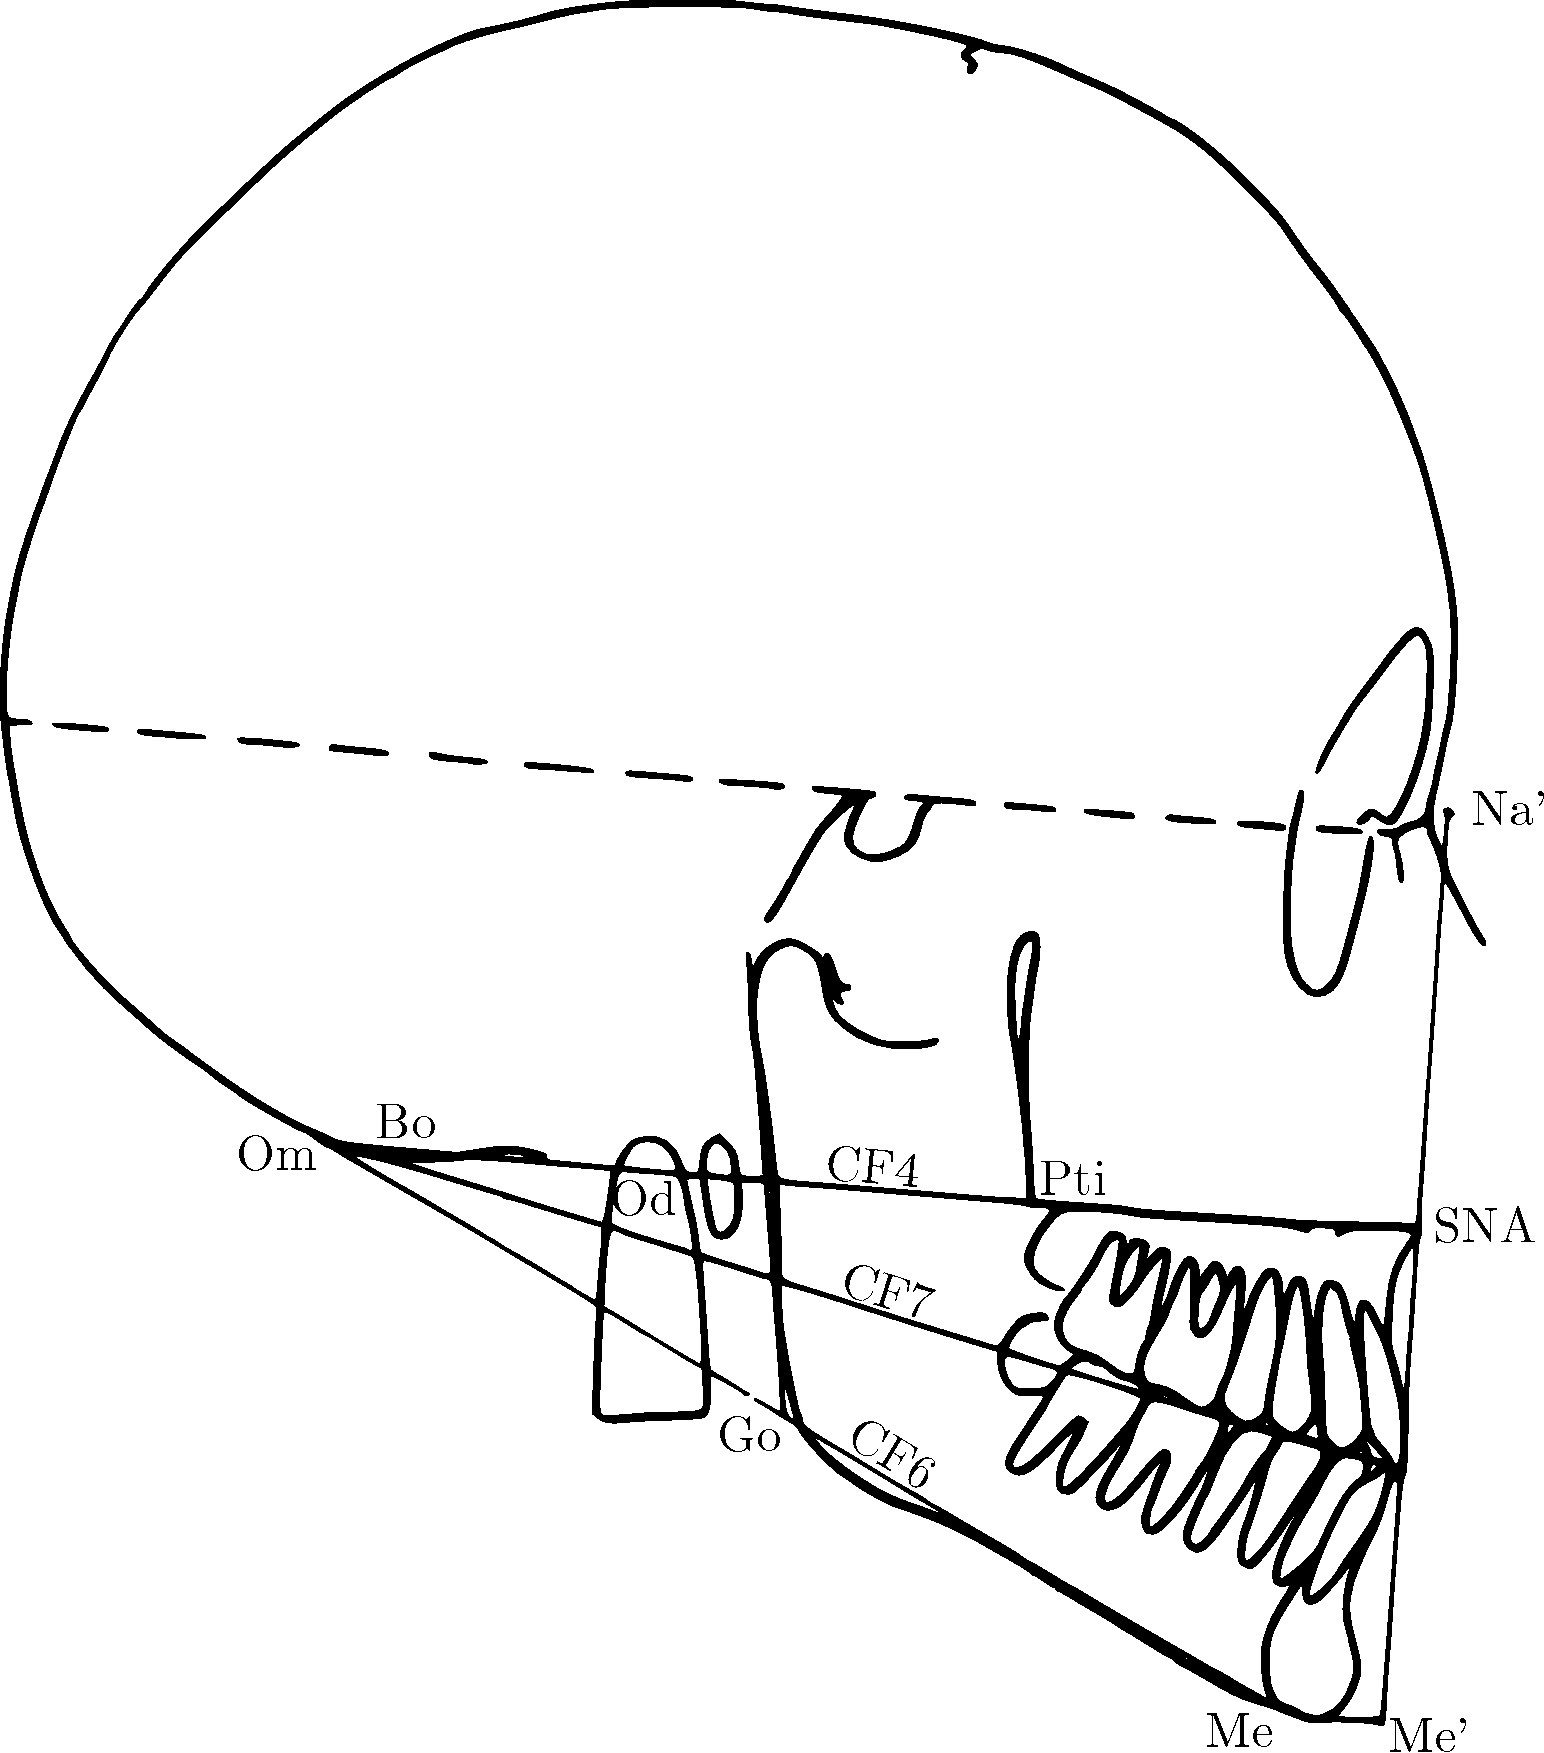
\includegraphics[width=.4\textwidth]{./images/delaire_bilancio_palatoocclusomandibolare.pdf}} \\
\subfloat[][]
   {\label{fig:delaire_bilancio_verticale}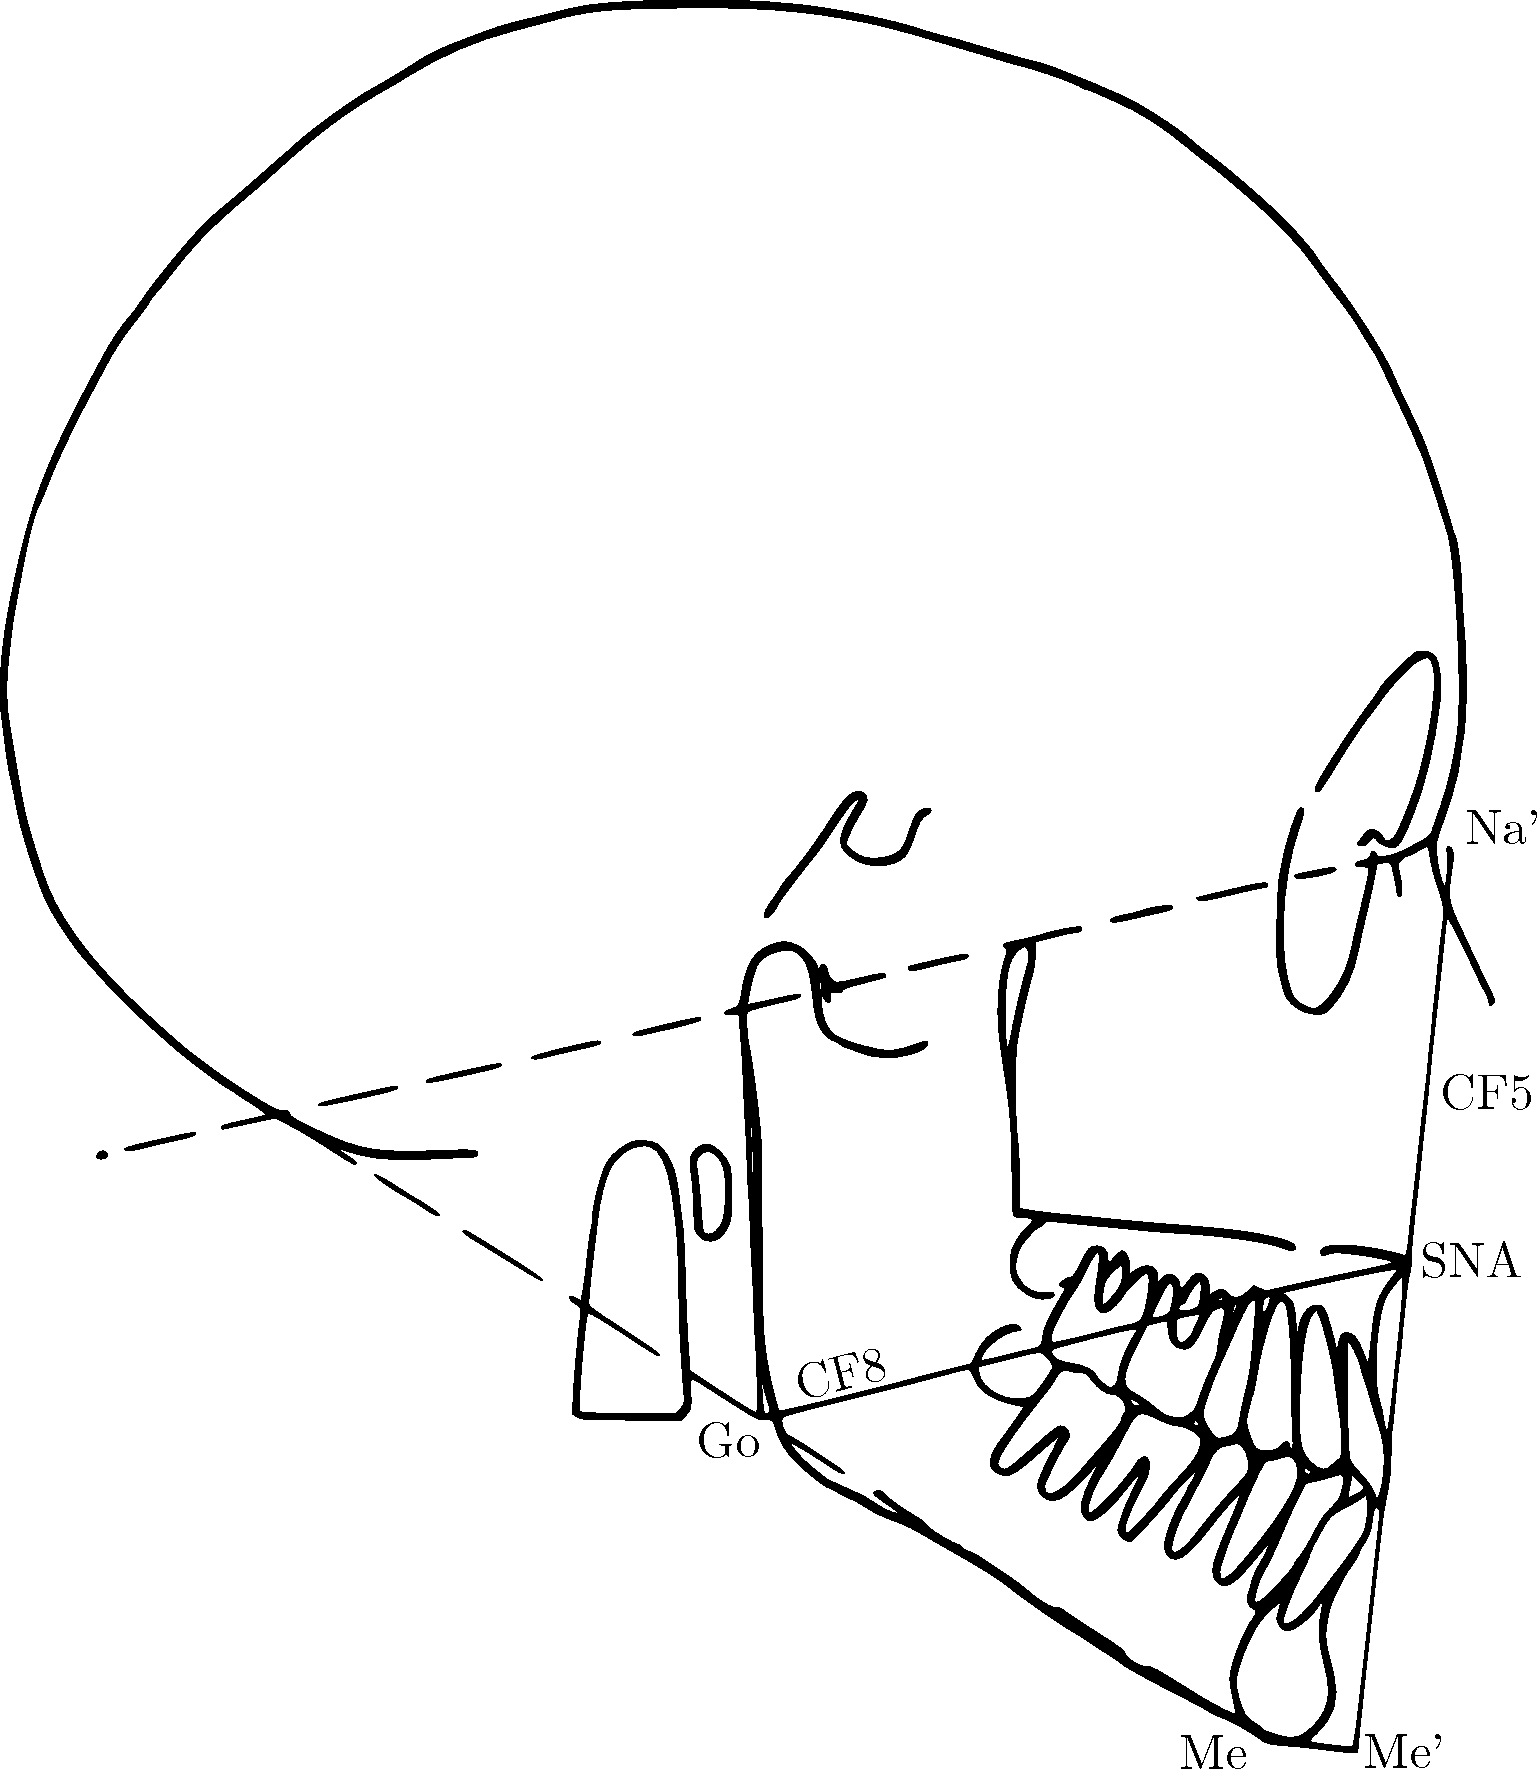
\includegraphics[width=.4\textwidth]{./images/delaire_bilancio_verticale.pdf}}
\caption{Linee facciali di Delaire: \subref{fig:delaire_bilancio_anteroposteriore} bilancio antero-posteriore; \subref{fig:delaire_bilancio_palatoocclusomandibolare} bilancio dei piani palatale, occlusale e mandibolare rispetto all'articolazione craniospinale; \subref{fig:delaire_bilancio_verticale} bilancio facciale verticale.}
\label{fig:delaire_facciali}
\end{figure}

Per analizzare la parte facciale vengono utilizzate otto linee, chiamate da \textbf{CF1} a \textbf{CF8}. Le prime tre (\textbf{CF1}, \textbf{CF2}, \textbf{CF3}) vengono utilizzate per studiare il bilancio antero-posteriore tra le strutture facciali e le strutture anteriori del cranio (figura \vref{fig:delaire_bilancio_anteroposteriore}); le linee \textbf{CF4}, \textbf{CF6} e \textbf{CF7} vengono usate per studiare l'equilibrio dei piani palatale, occlusale e mandibolare in relazione all'articolazione cranio-spinale e la parte postero-inferiore del cranio (figura \vref{fig:delaire_bilancio_palatoocclusomandibolare}); le linee \textbf{CF5} e \textbf{CF8} vengono usate per studiare il bilancio verticale anteriore e posteriore della faccia (figura \vref{fig:delaire_bilancio_verticale}).

\paragraph{Linea dell'equilibrio cranio-facciale anteriore} o \textbf{CF1}, viene tracciata perpendicolare a \textbf{C3}, passante da \punto{FMS}. Normalmente \textbf{CF1} si fonde con il pilastro mascellare anteriore che, da \punto{FMS}, segue la cresta lacrimale, scende al davanti del punto infraorbitario e quindi passa attraverso il bordo anteriore del forame superiore del canale nasopalatino. \\ Al di sotto del piano occlusale, \textbf{CF1} attraversa l'apice dell'incisivo centrale inferiore, e passa tra il terzo posteriore e il terzo medio della sinfisi mentoniera, arrivando al punto \punto{Me}. \\ Al di sopra di \textbf{C3}, divide la base del seno frontale in due parti uguali. \\ Queste condizioni sono ideali, ma non assolutamente necessarie, per un buon equilibrio facciale. Malgrado una rotazione di più o meno di 90° rispetto a \textbf{C3}, la faccia può essere ben equilibrata se tutti i punti tra \punto{FMS} e \punto{Me} sono posizionati sulla stessa linea. Un tale profilo dev'essere considerato normale, anche se non ideale. In particolare nelle donne e nei bambini, \textbf{CF1} risulta leggermente post-ruotato, con un angolo medio di 85°. \\ Un utile dato diagnostico ci è riferito dal \emph{punto di intersezione} tra il \textbf{CF1} ideale e la sinfisi mentoniera. Se interseca posteriormente, si può dire che la mandibola è grande; viceversa se interseca anteriormente. Questo dato è però strettamente dipendente dalla rotazione della mandibola: in caso di post-rotazione, \textbf{CF1} risulterà spostato in avanti.

\paragraph{Linea dell'equilibrio cranio-facciale media} o \textbf{CF2}, viene tracciata dal bregma \punto{Br} a \punto{Pts}, e viene estesa inferiormente fino all'intersezione col bordo inferiore della mandibola. Normalmente, questa linea passa da \punto{Pti} (punto pterigoideo inferiore), dato dall'intersezione tra l'asse della fessura pterigoidea e il bordo palatale superiore. Essa segue inoltre il bordo anteriore del ramo mandibolare, e interseca il piano mandibolare approssimativamente a metà tra \punto{Go} e \punto{Gn}. Se l'intersezione avviene più vicino a \punto{Go}, può indicare una protrusione mandibolare o un'ipermandibolia; se essa avviene più vicino a \punto{Gn}, può indicare una mandibola piccola o post-ruotata. \\ Il tratto \piano{Pts}{Pti} viene chiamato \emph{pilastro medio pterigoideo}.

\paragraph{Linea dell'equilibrio cranio-facciale posteriore} o \textbf{CF3}, viene costruita parallelamente a \textbf{CF2}, e tangenzialmente al bordo posteriore del condilo (\punto{Cp}). Normalmente questa linea è anche tangente al bordo posteriore della mandibola, e si fonde perciò con il \emph{pilastro posteriore mandibolare}. Nel caso questi non coincidessero, la causa è da ritrovarsi in una retrusione o protrusione mandibolare, in eccessi di sviluppo della zona dell'angolo mandibolare o in un'eccessiva inclinazione della branca montante con apertura dell'angolo.

\paragraph{Linea cranio-palatale} o \textbf{CF4}, viene tracciata parallelamente a \textbf{C3}, passante per \punto{SNA}. Solitamente, tale linea segue la superficie superiore del palato osseo, passa attraverso \punto{Pti}, la metà superiore dell'arco anteriore dell'atlante, al di sotto dell'apice del processo odontoide e arriva al punto di Bolton \punto{Bo}.\\
Nei bambini, questa linea è in posizione superiore rispetto agli adulti, in riferimento al processo odontoide. Questo è spiegato dal fatto che nel processo di crescita le vertebre cervicali si sviluppano più verso l'alto che verso il basso.\\
Quando nessun punto di riferimento cade sulla stessa linea, è necessario tracciare diverse linee, passanti per i diversi punti, andando a costituire una \emph{banda}: la linea di mezzo di questa sarà la linea presa come riferimento.
%\\
%Da CF4 risulta evidente la posizione della spina nasale anteriore, che può trovarsi verso l'alto, come nei morsi aperti, o verso il basso, nei morsi chiusi. La stessa sorte può subire la spina nasale posteriore che, a seconda dei movimenti della lingua, può orientarsi verso l'alto o verso il basso.

\paragraph{Altezza facciale teorica} o \textbf{CF5}, viene tracciata perpendicolare a \textbf{CF4}, passante per SNA. Su questa vengono proiettati perpendicolarmente il punto \punto{N} in \punto{N'}, e il punto \punto{Me} in \punto{Me'}. La distanza \piano{SNA}{Me'} è pari al 55\% di \piano{N'}{Me'}. Normalmente, la parallela a \textbf{CF4} attraverso \punto{Me'} interseca \textbf{CF1} nel punto \punto{Me} ideale. La posizione di \punto{Me'} può essere trovata raddoppiando la distanza \piano{N'}{SNA}, e aggiungendovi $\frac{1}{9}$ alla misura.\\
Solitamente, \punto{N'} è posizionato leggermente davanti a \punto{N}, e \textbf{CF5} passa quasi tangenzialmente agli incisivi centrali superiori.

\paragraph{Linea cranio-mandibolare} o \textbf{CF6}, è tangente alla squama dell'osso occipitale nel punto \punto{Om} (punto occipito-mandibolare), e passa dal punto \punto{Me} ideale di cui sopra. Normalmente questa linea segue il margine inferiore della mandibola, passando attraverso il punto \punto{Me}, e attraversando l'angolo mandibolare e \textbf{CF3} in \punto{Go}. In alcuni casi, la parte inferiore della squama dell'occipitale presenta modifiche tali che non può essere usata per tracciare questa linea; in questi casi sarà quindi necessario determinare l'altezza del ramo tracciando \textbf{CF8}, che normalmente interseca \textbf{CF3} in \punto{Go}, e la linea cranio-mandibolare verrà tracciata connettendo \punto{Me} a \punto{Go}.

%indica il piano mandibolare tracciato da \punto{Met} e tangente alla squama dell'occipitale. Incontra \punto{CF4} in un punto \punto{OM}. Questa linea indica lo sviluppo del bordo inferiore della mandibola, il grado dello sviluppo del ramo perlopiù diminuito nelle iperdivergenze, lungo per esempio in certe sindromi come l'acromegalia e in certi casi di \emph{long face} a ramo lungo. Evidenzierà anche il grado di post-rotazione mandibolare, il cui bordo eccederà dal piano mandibolare stesso.

\paragraph{Linea cranio-occlusale} o \textbf{CF7}, viene tracciata dal punto \punto{Om} al punto medio del tratto \piano{SNA}{Me'}. Di norma questa linea è tangente alle superfici occlusali dei premolari, e passa leggermente apicalmente ai margini incisali inferiori.

\paragraph{Altezza del ramo mandibolare} o \textbf{CF8}, viene tracciato parallelo a \textbf{C1}, passante per \punto{SNA}. Solitamente passa attraverso il gonion \punto{Go}.

\section{Analisi dentale}
\begin{table}[!ht]
\centering
%\footnotesize
\caption{Valori angolari dell'analisi dentale secondo Delaire}
\label{tab:delaire_dentale}
%\begin{tabular*}{.65\columnwidth}{lccc}
\begin{tabular}{lccc}
\toprule
 & CF4 & CF6 & Incisivo inferiore \\
\cmidrule(r){2-4}
Incisivo inferiore & --- & 90° & --- \\
Incisivo superiore & 110 $\pm$ 2° & --- & 135 $\pm$ 5° \\
\bottomrule
\end{tabular}
\end{table}

L'analisi dentale include lo studio dell'orientamento degli incisivi superiori e inferiori in relazione tra loro, e gli stessi in relazioni al piano mandibolare (\textbf{CF6}) e al piano palatale (\textbf{CF4}). I valori norma secondo Delaire sono schematizzati nella tabella \vref{tab:delaire_dentale}.